\documentclass[12pt,a5paper]{article}

\usepackage[T1]{fontenc} % font encoding, lubab õ tähte kasutada
\usepackage[utf8]{inputenc} % oleme siiski 21. sajandis, vajadusel on ka olemas utf8x
\usepackage{lmodern} % lmodern ja micrtype käivad käsikäes, teeb teksti ilusamaks
\usepackage{microtype}
\usepackage{tikz}
\usetikzlibrary{decorations.pathreplacing, positioning}
\usetikzlibrary{arrows,calc,decorations.markings,math,arrows.meta}

%\SIdecimalsign{,}
\usepackage{amsmath,amssymb} 
\usepackage{amsfonts}
\usepackage[estonian]{babel} % eesti keele poolitamisreeglid jpm
\usepackage[per = fraction, expproduct=cdot, decimalsymbol=comma]{siunitx} % http://www.bakoma-tex.com/doc/latex/siunitx/siunitx.pdf
\usepackage{graphicx} 
\usepackage{wrapfig}
\usepackage{epstopdf} %minul on vaja, et .eps pilte saada

%paneme kõik mõõdud paika
\topmargin=-2.5cm \textheight=18cm \textwidth=12.77cm
\oddsidemargin=-1.5cm  \evensidemargin=-1.5cm
\setlength{\parindent}{0pt} \setlength{\parskip}{6pt} \sloppy

\relpenalty=10000 \binoppenalty=10000 % Tekstisisestes valemites reavahetusi ärgu olgu


\pagestyle{empty} % ilma leheküljenumbrita

\newcommand{\numb}[1]{\vspace{5pt}\textbf{\large #1}}
\newcommand{\nimi}[1]{(\textsl{\small #1})}
\newcommand{\punktid}[1]{(\emph{#1~p.})}
\newcommand{\autor}[1]{\emph{ Autor: #1.}}
\newcounter{ylesanne}
\newcommand{\yl}[1]{\addtocounter{ylesanne}{1}\numb{\theylesanne.} \nimi{#1} \newblock{}}
\newcommand{\D}{\textrm{d}}

\tikzset{
	odot/.style={
		circle,
		inner sep=0pt,
		node contents={$\odot$},
		scale=2
	},
	otimes/.style={
		circle,
		inner sep=0pt,
		node contents={$\otimes$},
		scale=2
	},
	circ/.style={
		circle,
		draw,
		minimum size=3mm,
		inner sep=0
	},
	odot2/.style={
		circ,
		path picture={\fill circle[radius=1pt];}
	},
	otimes2/.style={
		circ,
		path picture={
			\draw (path picture bounding box.45) -- (path picture bounding box.225);
			\draw (path picture bounding box.135) -- (path picture bounding box.315);
		}
	}
}

\begin{document}

\begin{center}
\textbf{\large Eesti koolinoorte 30. füüsika lahtine võistlus} \vspace{3pt}

\emph{23. november 2019. a. Vanema rühma ülesannete lahendused}
\end{center}



\yl{RISTMIK} \punktid{6} \autor{Markus Rene Pae}

Kui Juku ja teise auto projitseeritu kaugus ristmikust ja kiirused on samad, siis nad jõuavad ristmikule täpselt sama ajaga $t = s/v = \SI{150}{\meter} / \SI{90}{\kilo\meter\per\hour} = \SI{150}{\meter} / \SI{25}{\meter\per\second} = \SI{6}{\second}$. Kui Juku saavuitaks hetkeliselt kiirenduse $a = \SI{0.5}{\meter\per\second\squared}$, siis selle ajaga jõuaks ta läbida $s = v_0 t + a t^2/2 = \SI{25}{\meter\per\second} \cdot \SI{6}{\second} + \SI{0.5}{\meter\per\second\squared} (\SI{6}{\second})^2 / 2 = \SI{159}{\meter}$. Seega on teise auto ristmikule jõudes autode vahemaa $\SI{9}{\meter}$. Nurk ei oma antud ülesandes tähtsust.



\yl{PUMPJAAM} \punktid{6} \autor{Valter Kiisk}

Olgu reservuaari pindala $S$. Vee mass on $m=\rho V=\rho h_0S$. Selle masskese on tõstetud kõrgusele $h=h_0/2$, seega potentsiaalne energia on $mgh=\frac{1}{2}\rho gh_0^2S$ ja energia pinnaühiku kohta
\[
w_s=\frac{1}{2}\rho gh_0^2\approx \SI{49}{\mega\joule\per\meter\squared}\approx\SI{13.6}{kWh\per\meter\squared}.
\]

Energiavajaduse rahuldamiseks on vaja keskmist energiatihedust
\[
w_t=\SI{100}{\kilo\watt\per\kilo\meter\squared}\cdot \SI{24}{\hour}=\SI{2400}{kWh\per\kilo\meter\squared}=\SI{0.0024}{kWh\per\meter\squared}.
\]
Otsitav suurus on ilmselt $w_t/w_s\approx \num{1.8e-4}$.



\yl{LÄÄTS} \punktid{8} \autor{Hans Daniel Kaimre}

Otsime kaugust $s$, mille korral tekib ekraanile reaalne kujutis, paneme kirja süsteemi jaoks läätse valemi:
$$\frac{1}{s}+\frac{1}{L-s}=\frac{1}{f}\Rightarrow \frac{L}{s(L-s)}=\frac{1}{f} \Rightarrow s^2-LS+Lf=0$$
Tegu on tavalise ruutvõrrandiga, kust saame, et $$s_{1,2}=\frac{1}{2}\big(L\pm\sqrt{L(L-4f)}\big)$$
Kuna $s$ on reaalne suurus, mitte imaginaarne, siis peab $L-4f \geq 0$, kust omakorda saame $f$ tingimuseks, et $f \leq L/4$. Seega kõige suurem võimalik fookuskaugus on $f = L/4$, mille korral saame $s_{1,2} = L/2$ ja suurenduse $M=s_2/s_1 = 1$ ehk kujutis on sama suur kui kujutist tekitav objekt.



\yl{LAETUD TASAND} \punktid{8} \autor{Kaarel Hänni}

Ühe laengu poolt tasandile avaldatav jõud on võrdne ja vastasmärgiline tasandi poolt laengule avaldatava jõuga. Seega on tasandile kokku mõjuv jõud 0 siis ja ainult siis, kui tasandi poolt laengutele avaldatud jõudude summa on 0. Tasandi elektriväli on konstantne ja risti tasandiga (ja tasandi eri pooltel erisuunaline). Seega on tasandi poolt laengutele avaldatud jõudude summa 0 siis ja ainult siis, kui kummalgi pool tasandit on võrdne arv laenguid. Laenguid on kokku paaritu arv, seega see on võimatu.



\yl{KUULID} \punktid{10} \autor{EFO Žürii}

Esimese kuuli kõrgus on \(h_1(t_0) = vt_0 - gt_0^2/2\) ja teise kuuli kõrgus \(h_2(t_0) = v(t_0-t) - g(t_0 - t)^2/2\), kui esimene kuul lastakse õhku, siis \(t_0 = 0\). Põrke hetkel on kuulide kõrgused võrdsed. Sellest saame avaldada põrkehetke \(t_0 = t_p\).
\begin{align*}
    vt_p - gt_p^2/2 &= v(t_p-t) - g(t_p -t)^2/2, \\
    vt_p - gt_p^2/2 &= vt_p - vt - gt_p^2/2 + 2gtt_p/2 - gt^2/2,\\
    gtt_p &= vt + gt^2/2, \\
    t_p &= v/g + t/2.
\end{align*}
Seda aega kasutades saame leida kummagi kuuli kiirused põrke hetkel. \(v_1 = v - gt_p = v - v - gt/2 = -gt/2\) ja \(v_2 = v -gt(t_p-t) = gt/2\) ehk \(v_p = |v_1| = |v_2|\). Seda saab ka tuletada energiajäävusest, et samal kõrgusel on kuulide kiiruste absoluutväärtused võrdsed. Elastse põrke korral kehtib nii impulsi kui ka energia jäävust, millest tuleneb, et võrdsete masside korral kuulide kiirused vahetuvad, ehk võrdsete vastassuunaliste kiiruste korral kiiruste suunad vahetuvad ja esimene kuul põrkab otse üles tagasi. Leiame kõrguse, kus toimus põrge
\[h_p = vt_p - gt_p^2/2 = v^2/g + vt/2 - g(v^2/g^2 + vt/g + t^2/4)/2 = v^2/2g - gt^2/8.\]
Pärast põrget tõusis esimene kuul veel kõrguse \(h_+ = v_p^2/2g = (gt/2)^2/2g = gt^2/8.\) Seega kuuli maksimaalne kõrgus pärast esimest põrget on \(h_p + h_+ = v^2/2g,\) mis oli ka esimese kuuli maksimaalne kõrgus enne põrget.

\textbf{Alternatiivne lahendus:} Kuna kuulid lastakse välja sama algkiirusel ning kokkuprge toimub ühel kõrgusel, siis energia jäävuse põhjal on kokkupõrke hetkel kuulide kiirused samad, kuigi vastassuunalised. Kui põrkuvad kokku kaks ühesugust kuuli samade kiirustega, siis energia ja impulsi jäävuse tõttu on peale kokkupõrget nende kiirused samad, mis enne, kuid vastupidise märgiga. Seetõttu saavutab esimene kuul jälle oma esialgse maksimaalse kõrguse, mis on $h=\frac{v^2}{2g}$.


\yl{LED} \punktid{10} \autor{Ardi Loot}

Valgusdioodid põlevad võimalikult heledalt, ja ei põle läbi, nimipingel
ja voolul. Pinge jaotumise kohta saab kirja panna võrrandi $U=I_{D}Z+NU_{D}$
ja seda lahendades leida vajaliku takisti ja kondensaatori näivtakistuse 
\begin{equation*}
Z=\frac{U-NU_{D}}{I_{D}}=\SI{2.9}{k\Omega}.
\end{equation*}
Kasutades takisti ja kondensaatori näivtakistuse valemit saame avaldada
vajaliku mahtuvuse
\begin{equation*}
C=\frac{1}{2\pi f\sqrt{Z^{2}-R^{2}}}\approx\SI{1.1}{\mu F}.
\end{equation*}


\yl{NIIT RELSSIDEL} \punktid{12} \autor{Jaan Kalda}

Olgu alumise rõnga kaugus nurgast $x$ ja vertikaalse rõnga kaugus $y$, niidi pikkus $L$ ja kinnituspunkti kõrgus $h$. Sellisel juhul $x^2+y^2=(L+y-h)^2$, võttes siit ajalise tuletise saame $2x\dot x+2y\dot y=2(L+y-h)\dot y$, kus punkt sümboli kohal tähistab ajalist tuletist, st $\dot x=v$. Lihtsustades seda avaldist leiame $vx=(L-h)\dot y$. Esiteks saame siit avaldada otsitava kiiruse
$$
\dot y=vx/(L-h)=v\left(\frac{L+y-h}{x-\frac yx}\right)^{-1}=
$$
$$
=v/(\frac 1{\cos\alpha}-\tan\alpha)^{-1}=\frac{v\cos\alpha}{1-\sin\alpha}.
$$
Teiseks, kui võtame antud avaldisest veelkord tuletise, saame $v\dot x=(L-h)\ddot y$, millest kiirendus $\ddot y=v^2/(L-h)$. Pangem tähele, et kiirendus püsib konstantne.


\yl{KÜLM GAAS} \punktid{12} \autor{Jaan Kalda}

Alghetkel lähenevad põhjale molekulid kiirusega $v$, seega lühikese ajavahemiku $t$ jooksul jõuavad põhjaga põrkuda molekulid ruumalast $vtS$, kus $S$ on põhja pindala, kogumassiga $\rho vtS$. Peale põrkumist lahkuvad nad kiirusega $v$ seetõttu said nad põhjalt koguimpulsi $\Delta p=2\rho vtS$. See vastab jõule $F=\Delta p/S$ ja rõhule $p=F/S=2\rho v$.

Pikema aja möödudes saavutavad molekulid soojusliku tasakaalu, st nende kiirusjaotus muutub isotroopseks ja algne kineetiline koguenergia muutub siseenergiaks: $U=V\rho v^2/2$, kus $V$ tähistab anuma ruumala. Teisest küljest, $U=\frac 32 \frac{\rho V}\mu RT$, millest $v^2=3 \frac{ RT}\mu$ ning $p=\frac{\rho}\mu RT=\rho v^2/3$.



\yl{HANTEL} \punktid{14} \autor{Jaan Kalda}

Tagamaks, et hantel on ekvipotentsiaalne, voolab pool laengust teisele kerale; see toimub väga kiiresti, sest varda takistus on tühiselt väike (eeldame, et $RC$-aeg on hulga väiksem tsüklotronperioodist). Laengu voolamise ajal mõjub vardale Ampère'i jõud $F=BL\frac {\mathrm d q}{\mathrm dt}$, kus $q$ tähistab teise kera laengut. Seetõttu on ülekantav jõuimpulss leitav kui $\Delta p=\int F\mathrm dt=\int BL\mathrm dq = BLQ/2$. Järelikult hakkab hantel liikuma kiirusega $v=\Delta p/2m=BLQ/4m$. Kuivõrd mõlema kuuli massid ja laengud on samad, siis hakkavad nad liikuma magnetväljas ühtmoodi, tsüklotronsagedusega $\omega=BQ/2m$ ja tsüklotronraadiusega $r=v/\omega=L/2$. Järelikult on kuulikeste trajektoorid ringjooned raadiusega $L/2$ ja diameetriga $L$, st tegemist on kahe üksteist puudutava ringjoonega.



\yl{LAME MAA} \punktid{14} \autor{Andres Põldaru}

Lennukist nähtav maakera horisont moodustab ringjoone. Selle ringjoone eri punktid asuvad kaamerast eri kaugustel. Millise kujutise kaamera sensorile tekitab ringjoon, mille erinevate punktide kaugus kaamerast on erinev?

Kõik kaamera vaatenurgas olevad ringjoone punktid on kaamerast väga kaugel. Kindlasti on lennukist näha kilomeetrite kaugusele, aga kaamera ise on väike. Seega on kõik horisondi punktid sisuliselt lõpmatuses ja võime heas lähenduses eeldada, et kaamera on nendele samaaegselt fokusseeritud. Kujutise leidmiseks tuleb kõik kiired projekteerida suvalisse tasandisse, mis on kaamera optilise peateljega risti.

Teeme joonise nr 1 maakera läbilõikega, kus Juku asub maakera kohal punktis $P$. Kaamera optiline peatelg on suunatud punkti $Q$. Olgu äärmine nähtav horisondi punkt $A$ ja selle projektsioon joonise tasandile $E$. Lennukist nähtava horisondi poolt moodustatud ringjoone keskpunkt on $O$. Projekteerime lennukist (punktist $P$) tõmmatud kiired tasandile, mis on optilise peateljega risti ja läbib punkti $E$.

Joonisel nr 2 on kujutatud horisondi ringjoont keskpunktiga $O$ eraldi, kus on näha äärmine nähtav punkt $A$ ja selle projektsioon $E$ eelmise joonise tasandisse. Heas lähenduses $\angle AOQ = \beta$, sest punktid $O$ ja $P$ on teineteisele lähedal ja pildi peal on punkti $A$ näha pildi servas peaaegu serva keskel (joonis 3). Täpselt pildi keskel on äärmiste punktide vahel $2\beta = \SI{60}{\degree}$.

\begin{center}
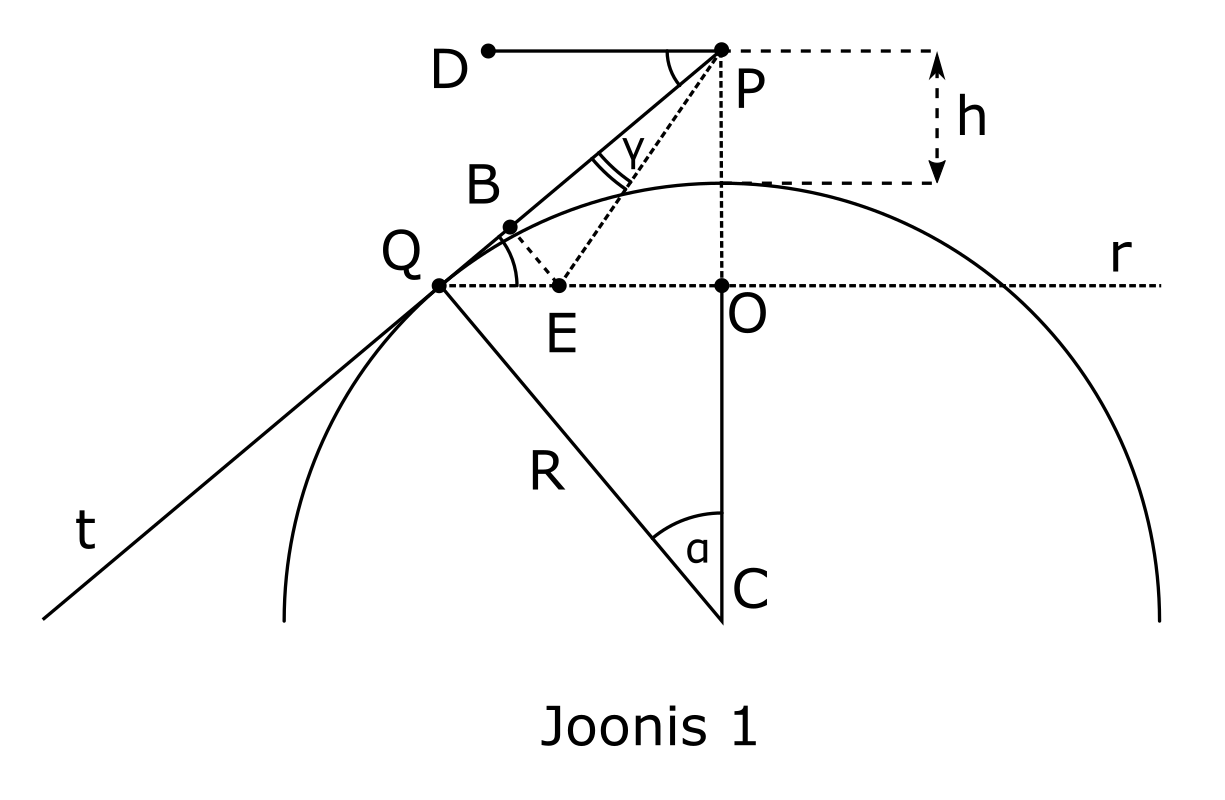
\includegraphics[width=0.50\textwidth]{joonis1}
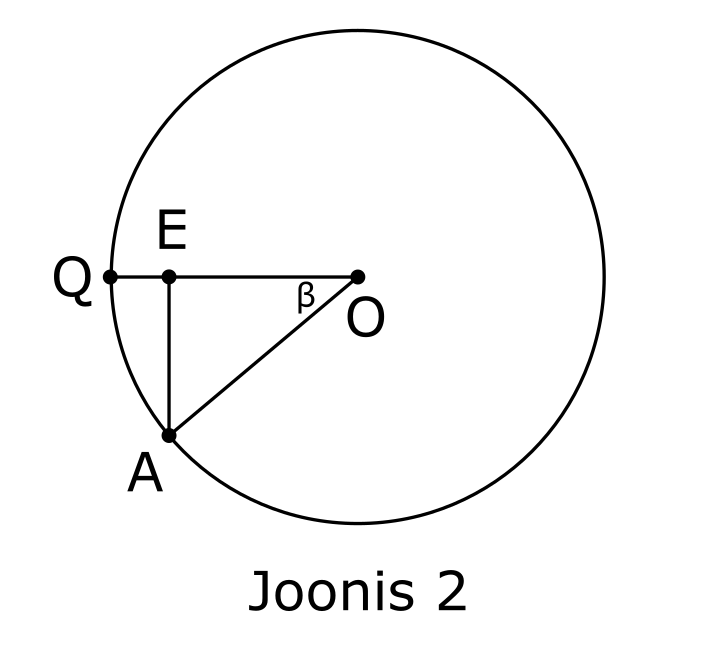
\includegraphics[width=0.265\textwidth]{joonis2}
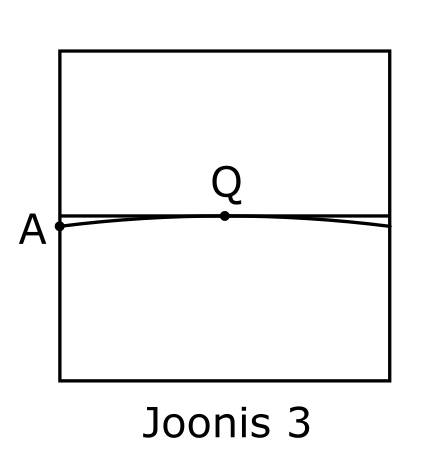
\includegraphics[width=0.215\textwidth]{joonis3}
\end{center}

Äärmise kiire projektsioon $|BE|$ vastab pildi peal üles-alla suunale. Seda projektsiooni iseloomustab nurk $\gamma=\SI{90}{\degree}-\alpha -\angle EPO$. 
Joonisel 1 leiame $$\cos{\alpha}=\frac{R}{R+h},$$ kust $$\alpha\approx\SI{3.3}{\degree}.$$ Veel leiame $$|OQ|=R\sin{\alpha}\approx \alpha R$$ ja $$|OP|=R+h-R\cos{\alpha}=\frac{h^2+2Rh}{R+h}\approx 2h.$$ Joonise 2 abil leiame $$|OE|=|OQ|\cos{\beta}\approx \alpha R\cos{\beta}.$$

Nüüd saame leida joonisel 1 nurga $\gamma$.
$$\gamma = \SI{90}{\degree}-\alpha-\angle EPO = \SI{90}{\degree}-\alpha-\arctan{\frac{|OE|}{|OP|}}\approx \SI{0.34}{\degree}.$$
Nurgale vastava suuruse pildil saame leida, arvestades, et poolele vaatenurgale $\beta=\SI{25}{\degree}$ vastab $\SI{5}{cm}$. Projektsioonid samasse optilise peateljega ristuvasse tasandisse on võrdelised vastavate projektsioonidega välja prinditud pildil. $$\frac{x}{\SI{5}{cm}}=\frac{\tan{\gamma}}{\tan{\beta}} \rightarrow x = \SI{0.64}{mm}.$$

{\bf Alternatiivne lahendus:} Joonistame vaatluspunktist $P$ maakerale $M$ puutujakoonuse $K$ ning olgu $M$ ja $K$ puutejoon ring $R$ keskpunktiga $O$. Olgu ringil $R$ punkt $Q$ pildivälja keskpunktiks. Tähistame punkti $Q$ läbiva $M$ puutujatasandi $t$-ga ning ringi $R$ poolt defineeritud tasandi $r$-ga. Olgu $r$ ja $t$ lõikejoon $T$. Teoreemist ringi puutujate kohta näeme, et $|PQ|=\sqrt{dh}$, kus $d$ on Maa diameeter ja $h$ - vaatluspunkti kõrgus. Seega nurk, mille all paistab Maa keskpunktist lõik $OQ$ on väikeste nurkade lähenduses $\alpha \approx 2|PQ|/d=2\sqrt{h/d}$ ning $|OP|\approx \alpha |PQ|=2h$. Märgime ringil $r$ punkti $A$ nii, et kaarele $QA$ vastav kesknurk oleks $\beta=25^\circ$; punkti $A$ kujutis asub pildi serval ning sirge $T$ kujutiseks on sirgjoon. Tõmbame punktist $A$ ristsirge tasandile $t$; tähistame selle ristsirge lõikepunkti tasandiga $t$ $B$-ga. Lõigu $AB$ kujutis pildil on meie otsitav suurus. Et punkti $A$ kaugus sirgest $T$ on $|OQ|(1-\cos\beta)$ ja tasandite $t$ ning $r$ vaheline nurk sarnaste kolmnurkade põhjal $\alpha \ll 1$, siis $|AB|\approx \alpha |OQ|(1-\cos\beta)\approx 2h(1-\cos\beta)$. Punkti $A$ kaugus sirgest $PQ$ omab ligikaudu pikkust $a=|OQ|\sin\beta$ ja kujutub pildi poollaiuseks $a'=\SI 5{cm}$.Järelikult kujutub lõik $AB$ lõiguks pikkusega $|AB|a'/a\approx a'\alpha(1-\cos\beta)/\sin\beta\approx 2a'\sqrt{h/d}(1-\cos\beta)/\sin\beta\approx \SI{0.64}{mm}$.




\end{document}